\begin{figure*}[t]
  \centering
  \subfloat[NRMSE with HotSpot.]{
    \label{fig:hotspot-error}
    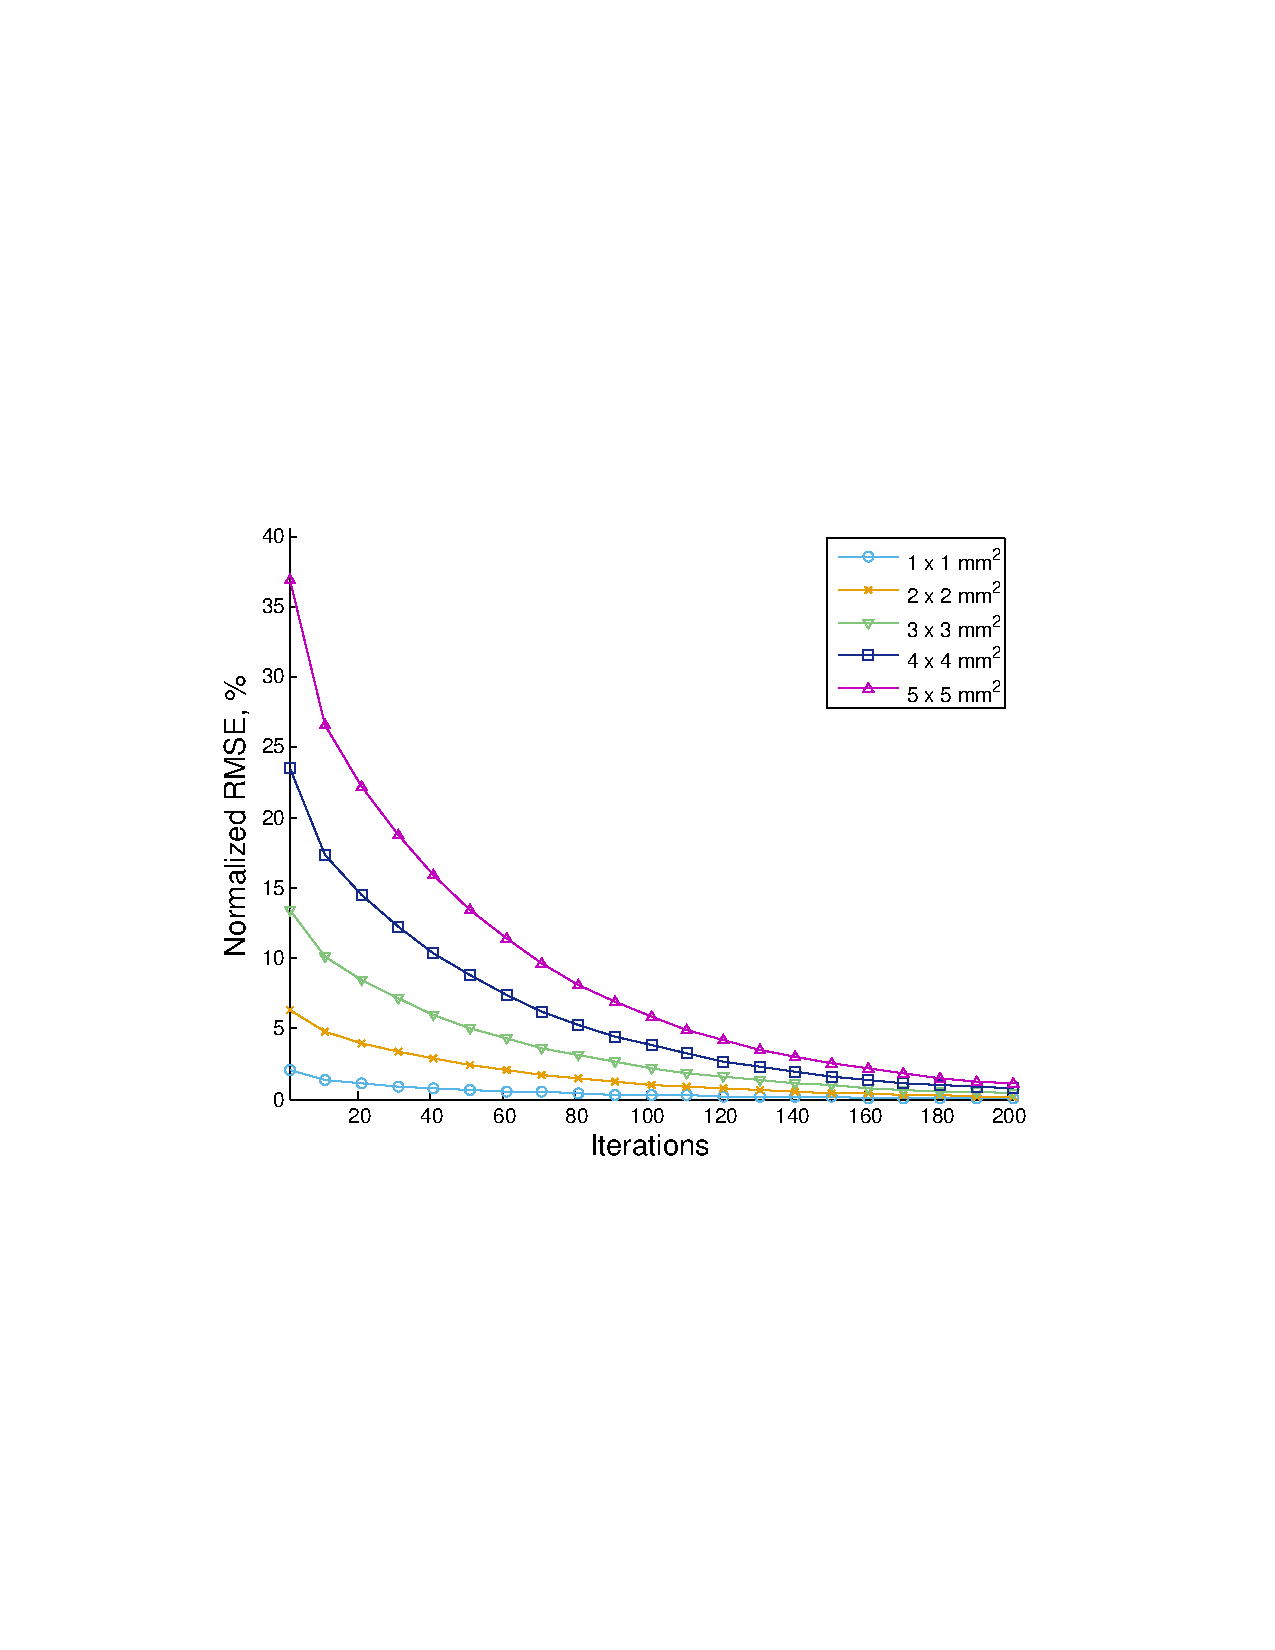
\includegraphics[width=0.32\linewidth]{assets/hotspot-error.pdf}
  }
  \subfloat[SSA with real SSDTP.]{
    \label{fig:steady-state-approximation}
    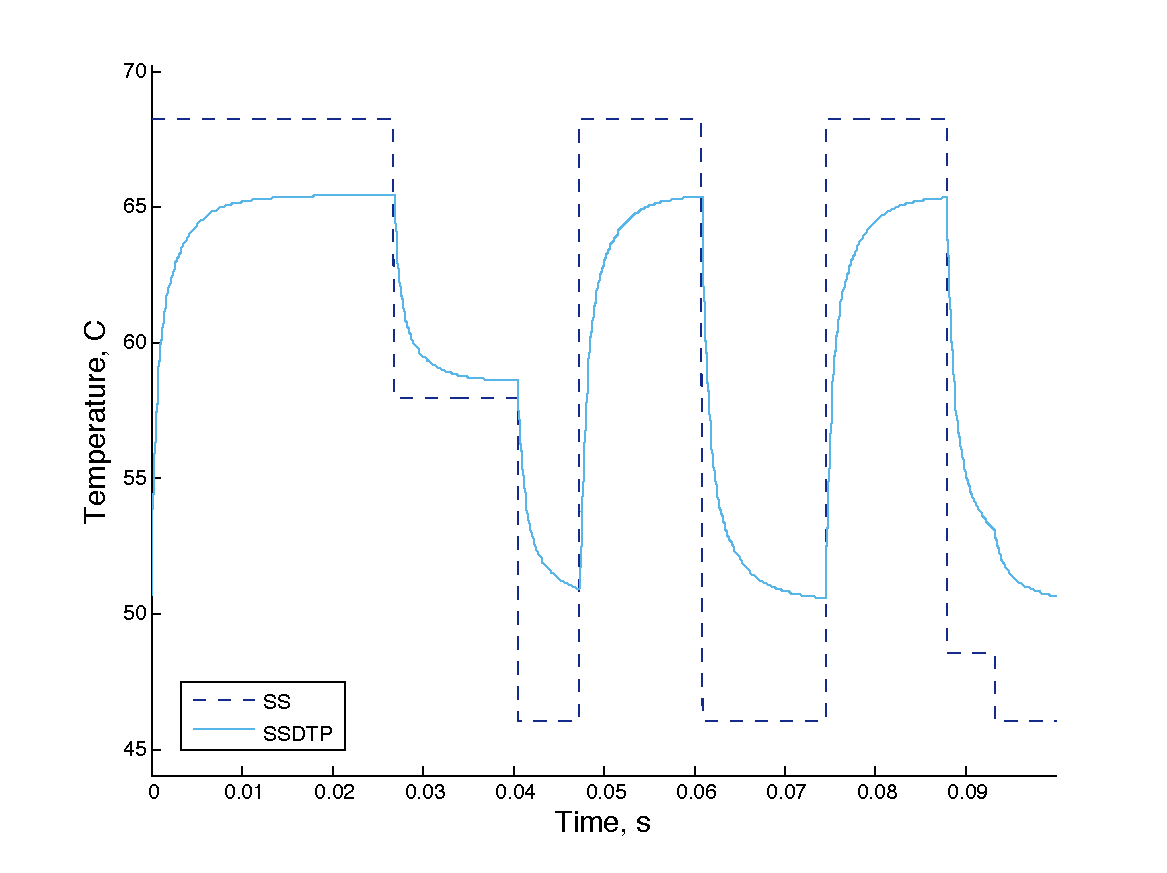
\includegraphics[width=0.32\linewidth]{assets/steady-state-approximation.pdf}
  }
  \subfloat[NRMSE with SSA.]{
    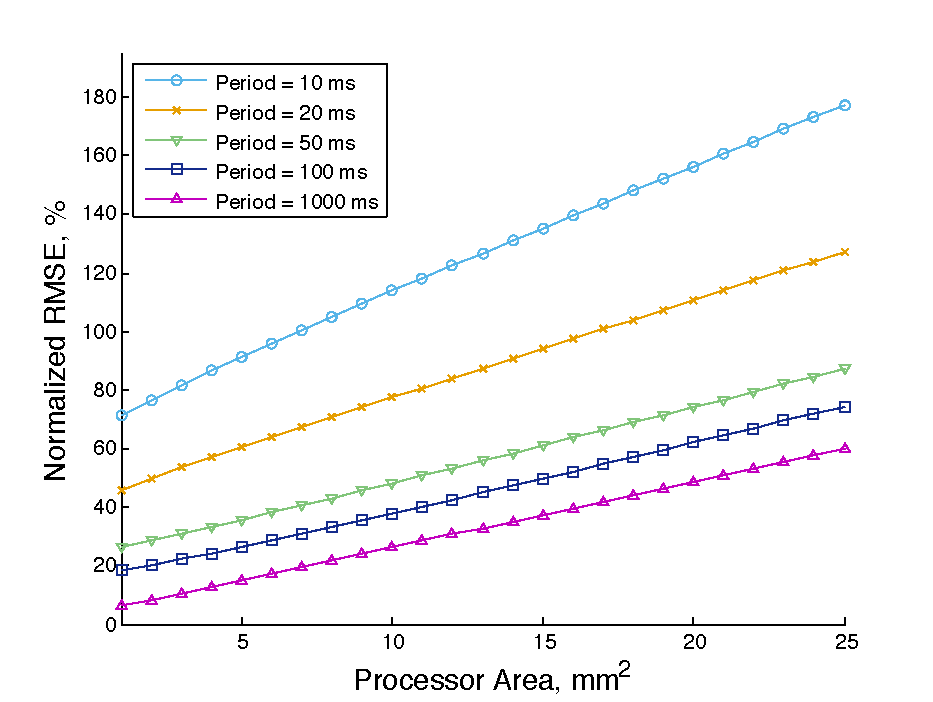
\includegraphics[width=0.32\linewidth]{assets/steady-state-error.pdf}
    \label{fig:steady-state-error}
  }
  \caption{State of the art solutions.}
\end{figure*}

\label{sec:architecture-model}
We consider a heterogeneous multicore architecture with a set of processing elements $\Pi$ defined as the following:
\[
  \Pi = \{ \pi_i = (V_i, \: f_i, \: N_{gate \: i}): \; i = \range{0}{N_p - 1} \}
\]
where $V_i$, $f_i$, and $N_{gate \: i}$ are the supply voltage, frequency, and number of gates \cite{liao2005} of the $i$th core, respectively.

\label{sec:power-model}
The total power dissipation of a processing element is defined as the sum of the dynamic and leakage power: $P = P_{dyn} + P_{leak}$. The dynamic part is modeled as $P_{dyn} = C_{eff} \cdot f \cdot V^2$ where $C_{eff}$ is the effective switched capacitance, $V$ and $f$ are the supply voltage and frequency, respectively. The leakage part of the power dissipation is defined as \cite{liao2005}:
\begin{equation} \label{eq:total-power}
  P_{leak}(T) = N_{gate} \: V \: I_0 \left[ A \: T^2 e^{\frac{\alpha \: V + \beta}{T}} + B e^{(\gamma \: V + \delta)} \right]
\end{equation}
where $T$ and $V$ are the current temperature and supply voltage, respectively, $N_{gate}$ is the number of gates in the circuit, $I_0$ is the average leakage current at the reference temperature and supply voltage. $A$, $B$, $\alpha$, $\beta$, $\gamma$, and $\delta$ are the technology-dependent constants found in \cite{liao2005}.

\label{sec:thermal-model}
Our proposed technique is based on the RC thermal model that employs the analogy between electrical and thermal circuits \cite{kreith2000}. Heat transfer is modeled with the following system of differential equations:
\begin{equation} \label{eq:fourier-model}
  \m{C} \: \frac{d\v{T}(t)}{dt} + \m{G} \: (\v{T}(t) - \v{T}_{amb})= \v{P}(t)
\end{equation}
where $\v{T}$ is the temperature vector, $\v{T}_{amb}$ is the ambient temperature vector, $\m{C}$ is the thermal capacitance matrix, $\m{G}$ is the thermal conductance matrix, and $\v{P}$ is the power dissipation vector. The dimensions of the system are \mbox{$N_n \times N_n$}, where $N_n$ is the number of nodes in the equivalent RC thermal circuit, which is further discussed in \appref{thermal-circuits}.
